% !TEX encoding = UTF-8
% !TEX TS-program = pdflatex
% !TEX root = ../tesi.tex

%**************************************************************
\chapter{Architettura per la comunicazione cross-page}
\label{cap:architettura}
%**************************************************************

In questo capitolo viene presentata prima l'architettura multi-process dei browser, in particolare di Chrome, per la gestione delle pagine web. Uno degli obiettivi è difatti la possibilità di eseguire i componenti nelle finestre figlie come processi separati, in modo da migliorare e non inficiare il processo dell'applicazione principale.

In seguito si illustra invece lo stato dell'arte delle diverse soluzioni per la comunicazione cross-page in JavaScript tra pagine su processi diversi e l'architettura finale utilizzata dalla libreria \textit{Stargate}.

\section{Architettura multi-processi}

Quando la maggior parte dei browser moderni fu progettata inizialmente, le pagine web erano semplici e avevano poco o nessun codice attivo. Per tale motivo, i browser renderizzano tutte le pagine usando lo stesso processo, al fine di mantenere basso l'utilizzo delle risorse. \\

Tuttavia, le pagine web odierne sono decisamente più attive a partire da siti statici ma con tanto uso di JavaScript fino a vere e proprie applicazioni web come Gmail. Grosse parti di queste applicazioni girano all'interno del browser, così come le normali applicazioni eseguono in un sistema operativo e, proprio come questi, il browser deve dunque tenere le applicazioni separate tra di loro. \\

Oltre a ciò, le parti del browser che renderizzano HTML, JavaScript e CSS sono diventate straordinariamente complesse nel corso del tempo. Diventa perciò palese che browser i quali pongono tutto il lavoro in un processo affrontano seri problemi di rubustezza, responsitività e sicurezza. \\

Se un'applicazione web causasse un crash nel rendering engine, porterebbe la terminazione anche delle altre pagine web aperte. Le applicazioni web inoltre competono reciprocamente per l'uso della CPU ed ognuna di esse è single-thread per design di JavaScript, per cui rischierebbero di diventare non responsive alle interazioni utente. Infine anche la sicurezza è un fattore in rischio poiché una pagina web potrebbe sfruttare vulnerabilità del browser per accedere a dati delle altre pagine nello stesso processo.

\subsection{Cosa fa ogni processo?}

\begin{figure}[H] 
    \centering 
    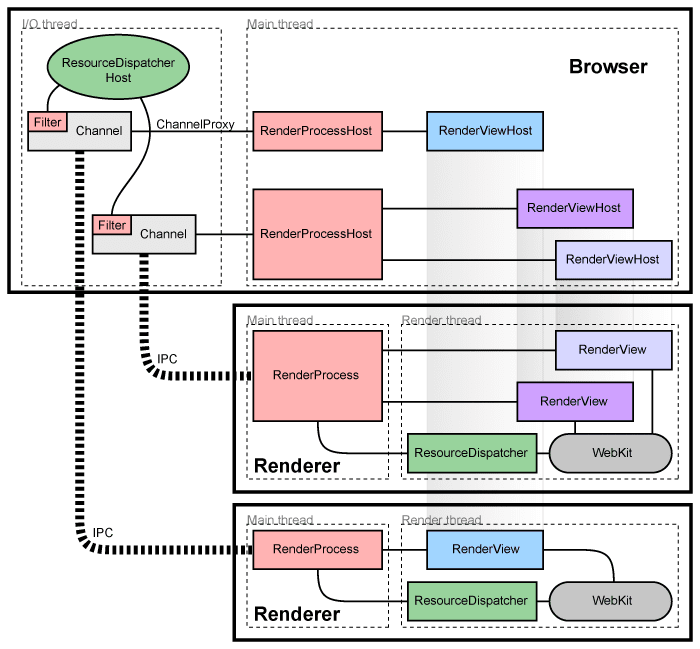
\includegraphics[width=1\columnwidth]{multi-process-arch} 
    \caption{Architettura multi-process in Chrome}
\end{figure}

Il browser crea tre differenti tipi di processi: browser, renderer ed estensioni.

\begin{itemize}
    \item \textbf{Browser}: esiste un unico processo browser, il quale gestisce i tab, le finestre e il browser stesso. Gestisce inoltre tutti i collegamenti delle pagine con il file system, la rete, input utente etc. ma non esegue alcun contenuto delle pagine;
    \item \textbf{Renderer}: il processo browser crea molteplici processi renderer, ognuno responsabile per la visualizzazione di una pagina web. I processi renderer contengono la complessa logica per la gestione di HTML, CSS, JavaScript, immagini e così via. Google Chrome, Safari ed altri utilizzano un rendering engine basato sul progetto open-source WebKit, mentre Firefox ed Edge hanno il proprio;
    \item \textbf{Estensioni}: il processo browser crea anche un processo per ogni estensione
\end{itemize}

\subsection{Strategie multi-process}

Una volta che il browser ha creato il processo omonimo, crea un processo renderer per ogni istanza di pagina web visitata dall'utente. Può essere pensato come un processo separato per ogni tab del browser, ma con l'eccezione di consentire a due tab di convidere lo stesso processo qualora siano collegati tra di loro e mostrino lo stesso sito. \\

Per esempio, se un tab ne apre un altro usando JavaScript o se viene aperto un link verso lo stesso sito in un nuovo tab, questi condivideranno lo stesso processo renderer. Si permette così ai tab correlati di comunicare via JavaScript e condividere la cache. Al contrario, se viene aperta una pagina di un sito diverso verrò riservato un nuovo processo. \\

Per essere precisi, si definisce un "sito" come un dominio registrato (ad esempio google.come o bbc.co.uk) e racchiude anche i sotto-domini (mail.google.com) e le porte (google.com:8080). Un' "istanza di sito" è invece un'insieme di pagine collegate provenienti dallo stesso sito. Due pagine sono considerate connesse se vi sono riferimenti reciproci in codice JavaScript, ad esempio una apre la seconda programmaticamente. Mentre se l'utente digita manualmente lo stesso indirizzo in due tab diverse, vengono considerate due istanze diverse con processi distinti. \\

Di seguito si illustrano nel dettaglio le diverse strategie multi-processi adottati dai browser moderni.

\subsubsection{Process-per-site-instance}

Normalmente i browser usano una strategia "Process-per-site-instance", ovvero lo stesso sito aperto in tab diversi con riferimenti reciproci saranno renderizzati dallo stesso processo. A volte è difatti necessario o desiderabile condividere il processo, quando per esempio un'applicazione web apre una nuova finestra con cui si aspetta di comunicare in maniera sincrona. \\

In generale invece, ogni nuova finestra o tab che non siano lo stesso sito possiede un nuovo processo.

\subsubsection{Process-per-site}

Raggruppa tutte le pagine dello stesso sito nello stesso processo, indipendentemente dalla presenza di riferimenti reciproci. Questa strategia è basata esclusivamente sul dominio del contenuto e non sulle relazioni tra le tab. Di conseguenza può risultare in processi molto onerosi.

\subsubsection{Process-per-tab}

Esiste anche una strategie più semplice che dedica un processo renderer per ogni gruppo di tab. Per ovvi motivi è estremamente inefficiente.
